\documentclass{beamer}
%%% BEGIN PREAMBLE

\usepackage{amsfonts}
% \usepackage{beamerthemesplit} // Activate for custom appearance

% Definitions
\theoremstyle{remark}
\newtheorem{remark}[theorem]{Remark}

\newcommand{\emptystring}{\varepsilon}
\newcommand{\length}[1]{\mid #1 \mid}
\newcommand{\directlygenerates}{\Rightarrow}
\newcommand{\generates}{\Rightarrow^{+}}
\newcommand{\generatesequal}{\Rightarrow^{*}}

\newenvironment{grammar}
	{\begin{tabular}[b]{lcl}}
	{\end{tabular}}
\newcommand{\rewritten}{$\to$}
\newcommand{\alternative}{$\mid$}

% Title stuff
\title{Formal Languages -- Basic Terminology}
\author{Peter Bauer}
\date{Version 01.02.02} % delete this line to display the current date

%%% BEGIN DOCUMENT
\begin{document}

\frame{\titlepage}

\begin{frame}
	\frametitle{Outline}
	\tableofcontents
\end{frame}

\section{Alphabet}
\begin{frame}
	\frametitle{Alphabet}
	
	\begin{definition}
		An {\em Alphabet} (sometimes called a {\em Vocabulary}) is a non-empty and finite set of elements.
	\end{definition}
	
	\begin{remark}
		Alphabets are often denoted by upper-case letters $A$ or $V$ and sometimes as upper-case greek letters like $\Sigma$.
	\end{remark}
	
	\pause
	
	\begin {example}
		\begin{itemize}
			\item $\{0, 1\}$: Binary alphabet.
			\item ASCII: Machine text alphabet.
			\item $\{a, b\}$: Small alphabet but enough for many examples.
		\end{itemize}
	\end{example}
\end{frame}

\section{String}
\begin{frame}
	\frametitle{String}
	\begin{definition}
		A {\em String} is a finite sequence of symbols of an alphabet.
	\end{definition}
	
	\pause
	
	\begin{remark}
		\begin{itemize}
			\item Strings are often denoted by lower greek letters like $\alpha, \beta, \varphi, \omega, \ldots$
			\item A string over the alphabet $\Sigma$ means a string all of whose symbols are in $\Sigma$.
		\end{itemize}
	\end{remark}
	
	\pause
	
	\begin{definition}
		The {\em length} of a string $\omega$ denoted as $\length{\omega}$ is the number of symbols
		in the string.
	\end{definition}
	
	\pause
	
	\begin{definition}
		A string  $\omega$ is called {\em empty} if $\length{\omega} = 0$. It is often denoted as $\emptystring$ or $\lambda$.
	\end{definition}
	
\end{frame}

\section{Concatenation}
\begin{frame}
	\frametitle{Concatenation}
	\begin{definition}
		Let $\omega_1$ and $\omega_2$ be two strings. The {\em concatenation} (sometimes also called {\em catenation})
		of $\omega_1$ and $\omega_2$ makes a new string $\alpha$ containing all the symbols of
		$\omega_1$ in order followed by all symbols of $\omega_2$ in order. This is usually written as
		$\alpha = \omega_1 \omega_2$.
	\end{definition}
	
	\pause
	
	\begin{example}
		Given two strings $\omega_1 = \mathtt{abc}$ and $\omega_2 = \mathtt{cde}$ then the concatenation $\alpha$ of
		$\omega_1$ and $\omega_2$ is
		$\alpha = \omega_1 \omega_2 = \mathtt{abc}\mathtt{cde}$.
	\end{example}
	
	\pause
	
	\begin{remark}
		For any string $\omega$ the relation $\emptystring \omega = \omega \emptystring = \omega$ holds.
	\end{remark}

\end{frame}

\section{Grammar}
\begin{frame}
	\frametitle{Production Rule}

	\begin{definition}
		A {\em production rule} (sometimes called a {\em re-writing rule} or simply {\em rule}) is a tuple
		$(A, \alpha)$, where $A$ is a symbol and $\alpha$ is a string of symbols.
	\end{definition}
	
	\pause
	
	\begin{remark}
	A rule is often denoted as $A \to \alpha$ and can be understood as "$A$ can be re-written (or substituted)
	by $\alpha$" or "$A$ is defined as $\alpha$".
	\end{remark}
	
	\begin{example}
		\begin{itemize}
			\item F \rewritten I
			\item I \rewritten a
		\end{itemize}
	\end{example}
\end{frame}

\begin{frame}
	\frametitle{Grammar}
	\begin{definition}
		A {\em grammar} $G(S)$ is a finite, non-empty set of production rules. $S$ is called the start
		symbol and appears on at least one left side of the production rules. All symbols on the left and
		right sides are the Vocabulary.
	\end{definition}
	
	\pause
	
	\begin{example}
		\begin{grammar}
			F & \rewritten & I \\
			F & \rewritten & $\lnot$F  \\
			F & \rewritten & (F $\land$ F)  \\
			F & \rewritten & (F $\lor$ F) \\
			I & \rewritten & a \\
			I & \rewritten & b \\
			I & \rewritten & c
		\end{grammar}
	\end{example}
\end{frame}

\begin{frame}
	\frametitle{Terminal and Non-Terminal Symbols}
	\begin{definition}
		All symbols appearing on the left side of a grammar $G(S)$ are called {\em non-terminals}. The set
		of all non-terminals of $G(S)$ is denoted by $V_N$. All other symbols are called {\em terminals}.
		The set of these symbols is denoted by $V_T$. Obviously it holds $V = V_N \cup V_T$.
	\end{definition}
\end{frame}


\begin{frame}
	\frametitle{Denoting Grammars --- Formal Languages}
	\begin {itemize}
		\item Terminals in lower-case letters
		\item Non-terminals in upper-case letters
		\item Separator: $\to$
		\item Alternatives: $\mid$
	\end{itemize}

	\pause
	
	\begin{example}
		The language of the propositional logic is defined as follows using the classical notation system
		of formal languages.
		
		\begin{grammar}
			F & \rewritten & I \alternative 
			 $\lnot$F  \alternative 
			(F $\land$ F)  \alternative 
			(F $\lor$ F) \\
			I & \rewritten & a \alternative b \alternative c
		\end{grammar}
	\end{example}
	
\end{frame}

\begin{frame}
	\frametitle{Denoting Grammars --- EBNF}
	\begin {itemize}
		\item Terminals under double quotes
		\item Non-terminals in meaningful words written in camel case
		\item Separator: $=$
		\item Alternatives: $\mid$
		\item Each rule ends with a period.
		\item Options: $[A]$ means $A$ or $\emptystring$.
		\item Repetition: $\{A\}$ means $\emptystring $ or $A$ or $AA$ or $AAA$ ...
		\item Parentheses for grouping.
	\end{itemize}

	\pause
	
	\begin{example}
		Expressions in the programming language Modula 2 written in EBNF.
		
		\begin{grammar}
			Expression & = & ["+" \alternative "-"] Term \{("+" \alternative "-") Term\}. \\
			Term & = & Factor \{("*" \alternative "/") Factor\}. \\
			Factor & = & c \alternative v \alternative "(" Expression ")".
		\end{grammar}
	\end{example}
\end{frame}

\begin{frame}
	\frametitle{Denoting Grammars --- Syntax Diagrams}
	\begin {itemize}
		\item Each diagram defines a non-terminal
		\item Terminals are represented by round boxes
		\item Non-terminals are represented by square boxes
	\end{itemize}
	
\end{frame}

\frame{
	\frametitle{Syntax Diagrams -- An Example}
	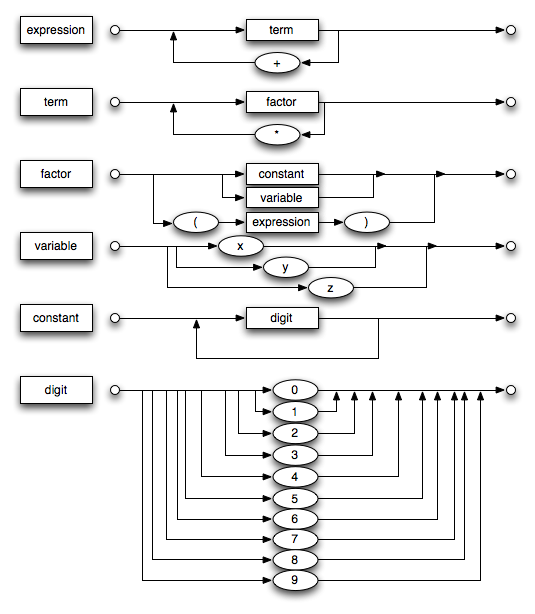
\includegraphics[scale=0.3]{SyntaxDiagrams.png}
}

\begin{frame}
	\frametitle{Syntax Trees or Parse Trees}
	
	Show by drawing the parse tree that  -5 + 3 * (a - x) is an expression in the sense of the grammar
	
			\begin{grammar}
			Expression & = & ["+" \alternative "-"] Term \{("+" \alternative "-") Term\}. \\
			Term & = & Factor \{("*" \alternative "/") Factor\}. \\
			Factor & = & c \alternative v \alternative "(" Expression ")".
		\end{grammar}

\end{frame}

\section{Generating Strings}
\begin{frame}
	\frametitle{Generating Strings}
	\begin{definition}
		Given
		\begin{enumerate}
			\item a formal grammar $G$ with a rule $A \to \varphi$
			\item a string $\alpha = \omega_1A \omega_2$.
		\end{enumerate}
		Then we can obviously generate a new string $\beta = \omega_1\varphi \omega_2$. In this case
		we say $\alpha$ {\em generates} $\beta$ {\em directly}, in symbols $\alpha \directlygenerates \beta$.
	\end{definition}
	
	\pause

	\begin{definition}
		A string $\alpha$ {\em generates} a string $\beta$ (usually denoted by $\alpha \generates \beta$ if
		there exists a sequence of direct generations
		\begin{equation*}
			\alpha = \omega_0 \directlygenerates \omega_1 \directlygenerates \omega_2 \directlygenerates \ldots \directlygenerates \omega_n = \beta.  \qquad (n > 0)
		\end{equation*}
		
		If $\alpha \generates \beta$ or $\alpha = \beta$ we write $\alpha \generatesequal \beta$ and say $\alpha$ {\em generates or is equal} to
		$\beta$.
	\end{definition}
\end{frame}

\section{Kleene Star and Language}
\begin{frame}
	\frametitle{Kleene Star}
	
	\begin{definition}
		Let $\Sigma$ be an alphabet. Then we define the sets $\Sigma_i$ recursively as follows:
		\begin{align*}
			\Sigma_0 & =  \{\emptystring\} \\
			\Sigma_{i + 1} & =  \{\omega\upsilon \mid \omega \in \Sigma_{i} \land \upsilon \in \Sigma\}
		\end{align*}
		
		The {\em Kleene star} is defined then by $\Sigma^* = \underset{i \in \mathbb{N}_0}{\bigcup}\Sigma_i$
	\end{definition}
	
	\pause
	
	\begin{example}
		Let $V = \{"\mathtt{ab}", "\mathtt{c}"\}$ be an alphabet. Then the $V^* = \{\emptystring, "\mathtt{ab}", "\mathtt{c}", "\mathtt{abab}", "\mathtt{abc}", "\mathtt{cc}", "\mathtt{cab}", "\mathtt{ababab}", "\mathtt{ababc}", \ldots\}$
	\end{example}
	
	\pause
	
	\begin{remark}
		Loosely interpreted we could say that the Kleene Star of an alphabet is the set of all strings that can be built out of this alphabet.
	\end{remark}
\end{frame}

\begin{frame}
	\frametitle{Language}
	\begin{definition}
		Let $G(S)$ be a grammar with a start symbol $S$. The set
		\[L(G(S)) =  \{\alpha: S \Rightarrow^* \alpha \land \alpha \in V_T^*\}\]
		is then called the {\em language} of $G(S)$.
	\end{definition}
	
	\pause
	
	\begin{example}
		Let $G($Java$)$ be the grammar defining the programming language Java. $L(G($Java$))$ is then
		\pause
		the set of all syntactically correct Java programs.
	\end{example}
\end{frame}
\end{document}
